\begin{figure}[t]
    \centering
    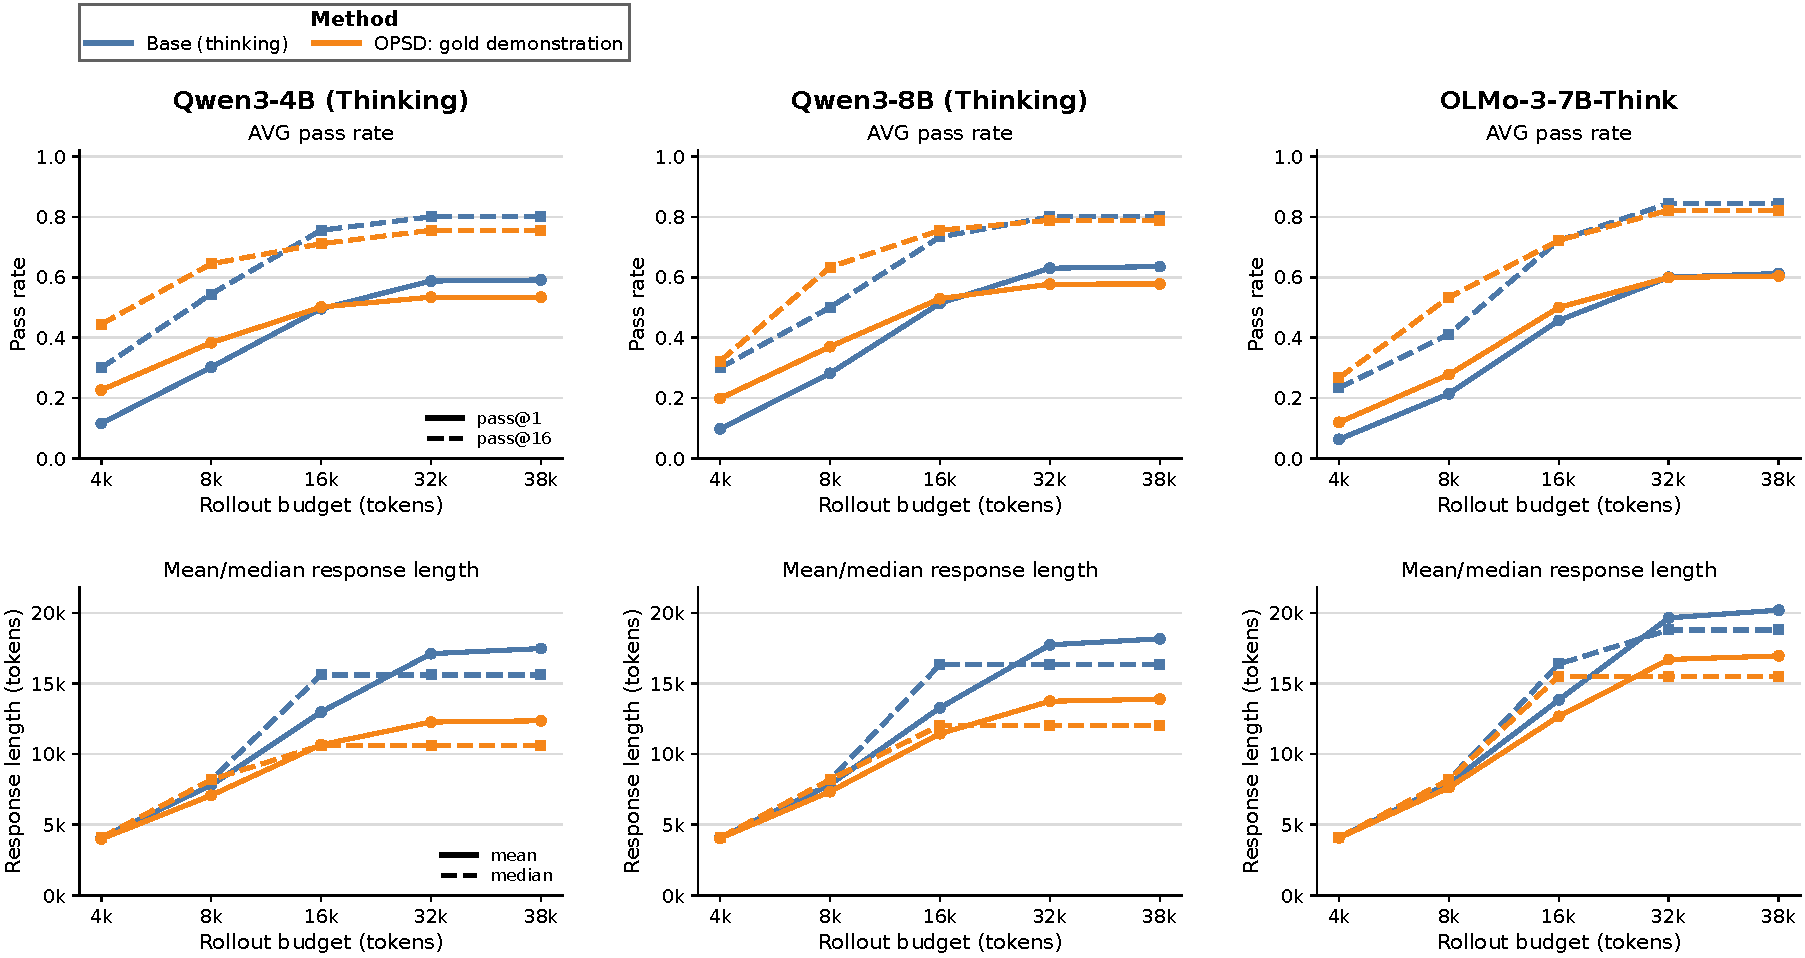
\includegraphics[width=\linewidth]{figures/avg_pass_and_rollout_tokens_qwen_olmo_demo_only.pdf}
    \caption{
    \textbf{For thinking models, \opsd{} can improve short-budget performance via compression but can hurt long-budget reasoning.}
    We evaluate OpenThoughts-trained Qwen3-4B, Qwen3-8B, and OLMo-3-7B thinking models across rollout budgets. Models are trained with a 4,096-token completion cap and evaluated at generation caps from 4,096 to 38,912 tokens. Top row: pass@1 and pass@16, averaged over AIME24, AIME25, and HMMT25. Bottom row: mean and median response length. \opsd{} with gold demonstrations often helps at 4k--8k tokens, but the advantage shrinks or reverses at 32k--38k tokens, where responses become substantially shorter than the base model.
    }
    \label{fig:openthoughts_accuracy_length_collapse}
\end{figure}
